\documentclass{homework}

\usepackage{enumitem}
\usepackage{tcolorbox}

\usepackage{tikz}
\usetikzlibrary{positioning,calc}

\usepackage{listings}

\lstset{
basicstyle=\small\ttfamily,
columns=flexible,
breaklines=true
}

\usepackage{fancyvrb}
\fvset{listparameters=\setlength{\topsep}{0pt}\setlength{\partopsep}{0pt}}

\title{02}

\begin{document}
\maketitle

\textbf{Organisational details}

\begin{itemize}
  \item Include in your report approximately how long the homework took you.
  \item You must follow the submission instructions outlined on GitLab.
  \item If the GitLab pipeline does not succeed, I will not grade your assignment (you will receive 0).
  The same applies if the Markdown report is illegibly formatted or if you miss the final submission deadline.
  \item I will provide feedback on Discord and/or GitLab.
  Check both after receiving your grade.
  \begin{itemize}
    \item My initial feedback may be quite minimal as there are so many of you.
    However, you can request additional feedback.
    Specific questions are also welcome.
    \item Do not share the feedback you receive, as this may give others an unfair advantage.
  \end{itemize}
  \item Grace clause submission deadline: 07.03.2026 23:59 EET.
  \begin{itemize}
    \item The grace clause applies only if you submit the full work (all tasks) by the soft deadline and the GitLab pipeline succeeds.
    \item You have one week from receiving the feedback to fix and resubmit your improved work.
    You may regain up to (but not necessarily) half of the lost points.
  \end{itemize}
  \item You may share hints with each other, but not answers or code.
  Ask questions in the server if they could benefit everyone.
  \item You may -- and I encourage you to -- ask me questions.
  \item You may use AI as assistance, but not to solve the tasks themselves.
  \begin{itemize}
    \item Acceptable: e.g. checking your understanding, asking how to loop in Python.
    \item Not acceptable: e.g. generating code logic, library use, or crypto operations.
    \item If you use AI in any form, including for rewording, state in your report where and what you used it for.
    \item I recommend asking in the server or contacting me instead of using AI.
  \end{itemize}
  \item If I catch you plagiarising, copying, or using AI for code logic, I will report you to the faculty and fail you for the course.
  \begin{itemize}
    \item If during the exam you are unable to explain material for which you received homework credit, I may ask you to explain your work.
    \item If you cannot convince me that the homework is your own work, I will report you to the faculty and fail you.
  \end{itemize}
\end{itemize}

\newpage

\begin{center}
  Theory tasks
\end{center}

\textbf{Additional instructions}

\begin{itemize}
  \item \textbf{Please do not use AI for the theoretical part.}
  Challenge your understanding and look for additional written sources if the lecture and provided materials are not enough.
  Critical thinking and clear communication are skills -- use them or lose them.
  \item You must reference all external materials you rely on, including AI tools, if you choose to use them anyway.
\end{itemize}

\begin{task}{Time to digest}
  You are given two pieces of data $d_1$ and $d_2$.
  You are also given $h_1 = H(d_1)$ and $h_2 = H(h_1||d_2)$, where $H$ is a cryptographic hash function.

  Does this prove that $d_1$ was created before $d_2$?
  Explain why or why not.
\end{task}

\begin{task}{Domain Separation}
  Read the following material:
  \begin{itemize}
    \item \href{https://gotchas.salusa.dev/domain_separation.html}{\textit{CryptoGotchas}} -- domain separation
    \begin{itemize}
      \item From the beginning until the section \enquote{Different Keys} (inclusive)
      \item The section \enquote{Final Thoughts}
    \end{itemize}
    \item \href{https://datatracker.ietf.org/doc/html/rfc5869#section-3.2}{RFC 5869} (HKDF), Section 3.2
  \end{itemize}

  Why is domain separation needed between leaf and internal node hashes in Merkle trees?
  Describe a concrete attack that becomes possible without it.\\
  {\scriptsize Vague statements like \enquote{because of security} or \enquote{for second preimage resistance} are not answers.}

  {\scriptsize Hint: See Section 2.1.1 of \href{https://datatracker.ietf.org/doc/html/rfc9162#section-2.1.1}{RFC 9162}.
  The \href{https://crypto.stackexchange.com}{Cryptography Stack Exchange} has some relevant posts as well.
  Reference any posts you use.}
\end{task}

\begin{task}{Input collision}
  While collision attacks should not be feasible against a cryptographic hash function, it is still possible to introduce collision vulnerabilities through improper use.

  Consider the construction
  \[
    H(x, y) \defeq H(x||y)
  \] where $x, y$ are variable-length inputs, i.e. their length is not fixed.

  Explain why this construction may be unsafe (barring length-extension).
  Give an example.

  {\scriptsize Input collisions and length-extensions are examples of canonicalisation attacks.
  See Soatok's blog post on \href{https://soatok.blog/2021/07/30/canonicalization-attacks-against-macs-and-signatures/}{\textit{Canonicalization Attacks Against MACs and Signatures}} for more.}
\end{task}

\newpage
\setcounter{task}{0}

\begin{center}
  Practical tasks
\end{center}

\textbf{Additional instructions}

\begin{itemize}
  \item I must be able to run your program with Python 3.14 and OpenSSL v3.6.1\footnotemark{}.
  \footnotetext{You may use older versions of Python and OpenSSL as long as they are interoperable with mine.}
  \item The GitLab pipeline must succeed before you submit your assignment.
  \item You may not import any third-party module other than \texttt{cryptography}, \texttt{requests}.
  You are free to import any built-in module.
  If you feel the need to import another third-party module, please check with me beforehand!
  \item All errors must be handled: print a descriptive message starting with \enquote{Handled:} and exit with error code \texttt{1}.
  Filesystem errors (e.g. file read/write errors) need not be handled.
  \item You must identify potential edge cases yourself.
  You may not ask an AI to implement them or identify them for you.
  \item You may change anything in the template files, unless specified otherwise, as long as the GitLab pipeline succeeds.
\end{itemize}

\begin{task}{Proof of work}
  Task template file: \texttt{merkle\_submit\_template.py}

  \textit{Background.}
  The core idea behind a proof of work (PoW) is to prove that you have expended some amount of computational effort.
  In essence, it is a puzzle that is computationally costly to solve, but the solution of which is easy to verify (similarly to the desired asymmetry in public-key cryptography).

  In this task, you must implement a simple variant of the \href{https://en.wikipedia.org/wiki/Hashcash}{\textit{Hashcash}} proof-of-work system, which is used for example in Bitcoin mining.
  You may (but need not) read more about Bitcoin's proof of work \href{https://en.bitcoin.it/wiki/Proof_of_work}{\textit{here}}.

  \textit{Context.}
  This task is closely coupled with the next task.
  I have implemented an append-only ledger to which you can submit up to 255-byte long strings.
  In order to commit data to the ledger, you must additionally send a Proof of Work associated with that data.

  In this task, you implement the proof of work and commit data to the ledger.
  In the next task, you prove that your data was included in the ledger.

  If you cannot complete this task, you may use a leaf node created by someone else for the next task.

  \textit{Instructions.} Implement the function
  \begin{Verbatim}
l0_bits(bs: bytes) -> int
  \end{Verbatim}
  that counts the number of leading 0 bits in the byte string and returns it.
  Since this is part of the code logic, you may not ask an AI to generate it for you.

  Implement the function
  \begin{Verbatim}
bruteforce(seed: bytes, difficulty: int) -> tuple[int, bytes]  
  \end{Verbatim}
  that iteratively generates 4-byte nonces until the hash value \texttt{SHA512/256(seed||nonce)}
  starts with at least 25 zero-bits (the challenge \enquote{difficulty}). That is, you try for nonces:
  \begin{enumerate}
    \item \texttt{0x00000000}
    \item \texttt{0x00000001}
    \item \texttt{0x00000002}
    \item \dots
  \end{enumerate}

  For example, for the seed \texttt{takraa}, the smallest integer nonce that produces the desired hash is $86197437$.
  Indeed, the hex value of this integer is \texttt{0x00000000052344bd}, and
   \begin{Verbatim}
SHA512/256(b"takraa\x00\x00\x00\x00\x05\x23\x44\xbd")
  \end{Verbatim}
  yields the hash value
  \begin{Verbatim}
00000060c45f26ecd9d97c05571088b77ccaed193f5723b7fd526982b5b0eebc
  \end{Verbatim}
  the first 25 bits of which are \enquote{0}.

  The function must work also for higher and lower difficulty settings, and must treat possible edge cases.

  In the \texttt{main()} function, set \texttt{data} to some string ($0<x\le255$) bytes in length, and set $\texttt{uni\_id}$ to your Uni-ID (i.e. your student username).
  Take note of the server's (successful) response, as you will need it for the next task.
\end{task}

\newpage

\begin{task}{Proof of inclusion}
  Task template file: \texttt{merkle\_proof\_template.py}

  In this task you will generate a \emph{Merkle inclusion proof} for a leaf in a Merkle tree.

  This task might appear daunting at first.
  Approach it in a \enquote{divide and conquer} manner and work it out on paper first.
  Draw a small tree and observe the pattern for determining the left-right sibling order by progressively adding more nodes.

  Implement the function
  \begin{Verbatim}
get_merkle_proof(
        tree: list[list[bytes]],
        leaf_index: int
) -> list[tuple[Literal["left", "right"], bytes]]
  \end{Verbatim}

  \textit{Input format.}
  The first argument contains the Merkle tree represented as a list of levels:
  \begin{itemize}
    \item The outer list contains the levels of the tree.
    \item Each inner list contains the hashes of the nodes at that level.
    \item The first level contains the leaves.
    \item The last level contains the root.
  \end{itemize}

  For example, the tree
  \begin{figure}[h]
      \centering
      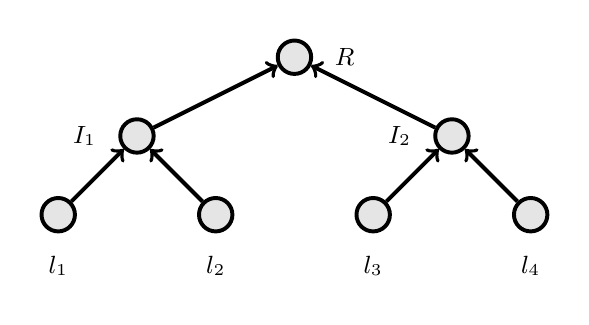
\begin{tikzpicture}
        [level distance=10mm,
        every node/.style={fill=gray!20,draw=black,circle,line width=0.5mm,inner sep=1.5mm},
        edge from parent/.style={<-,draw},
        level 1/.style={sibling distance=40mm,line width=0.5mm,nodes={fill=gray!20}},
        level 2/.style={sibling distance=20mm,nodes={fill=gray!20}},
        level 3/.style={sibling distance=10mm,nodes={fill=gray!20}}]
        \node[label={right:\small $R$}] {}
            child {node[label={left:\small $I_1$}] {}
              child {node[label=south:{\small $l_1$}] {}}
              child {node[label=south:{\small $l_2$}] {}}
            }
            child {node[label={left:\small $I_2$}] {}
              child {node[label=south:{\small $l_3$}] {}}
              child {node[label=south:{\small $l_4$}] {}}
            };
        \end{tikzpicture}
  \end{figure}
  
  is represented as
  \begin{Verbatim}
[[l1, l2, l3, l4], [I1, I2], [R]]
  \end{Verbatim}

  The second argument specifies the index of the leaf for which you must generate an inclusion proof.
  \begin{tcolorbox}[title=NB!]
    The leaf identifiers start with the number $1$, but indexes start at $0$.
  \end{tcolorbox}

  \textit{Output format.}
  The function returns a list of nodes that allow a verifier to recompute the root hash from the leaf.

  Each element of the proof must be a tuple of the form

  \begin{Verbatim}
("left" | "right", sibling_hash)
  \end{Verbatim}

  The direction indicates whether the sibling node lies to the left or to the right of the node whose hash you are currently computing.
  Examples:
  \begin{itemize}
    \item E.g. a proof for $l_2$ linking to $I_1$:
    \begin{Verbatim}
[("left", l1)]
    \end{Verbatim}

    \item E.g. a proof for $l_2$ linking to $R$:
    \begin{Verbatim}
[("left", l1), ("right", I2)]
    \end{Verbatim}

    \item E.g. a proof for $l_3$ linking to $R$:
    \begin{Verbatim}
[("right", l4), ("left", I1)]
    \end{Verbatim}
  \end{itemize}

\textit{Perfect roots.}

  Your proof must link the leaf to a \emph{perfect root} on the leftmost branch.
  I call \enquote{perfect root} the root of a perfect binary subtree, i.e. a subtree that contains a number of leaves that is a power of two.

  For example, in the tree
  \begin{Verbatim}
[[l1, l2, l3, l4], [I1, I2], [R]]
  \end{Verbatim}

  the following nodes are perfect roots on the leftmost branch.

  \begin{itemize}
    \item $I_1$ (covers leaves $l_1,l_2$)
    \item $R$ (covers leaves $l_1,l_2,l_3,l_4$)
  \end{itemize}

  While $I_2$ covers leaves $l_1, l_2$, it was never a root of the full tree.

  If the tree had three leaves $l_1,l_2,l_3$, then

  \begin{itemize}
    \item $I_1$ would be a perfect root (covers $l_1,l_2$)
    \item $R$ would not be a perfect root because the subtree contains $3$ leaves
  \end{itemize}

  In this case you cannot yet create a proof for $l_3$, because it does not belong to any perfect subtree rooted on the leftmost branch.
  You can either remediate this by inserting new leaves yourself, or wait until other students submit their leaves.

  This simulates the publishing of perfect roots in widely witnessed evidence, which is why the proof must link to them.
  Your proof must not necessarily link to the latest root if there are older perfect roots that can be linked to.

  \textit{Filling the tree.}
  The tree follows the Trillian / Certificate Transparency construction (see the week 5 practice).

  In my implementation:
  \begin{itemize}
    \item Leaf hashes are computed as
    \begin{Verbatim}
SHA512/256(0x00||data)
    \end{Verbatim}

    \item Internal node hashes are computed as
    \begin{Verbatim}
SHA512/256(0x01||left_node||right_node)
    \end{Verbatim}

  \item If a node has no partner (because the level contains an odd number of nodes), it is promoted unchanged to the next level.
\end{itemize}

  For example, a tree with three leaves looks as follows:
    \begin{figure}[h]
      \centering
      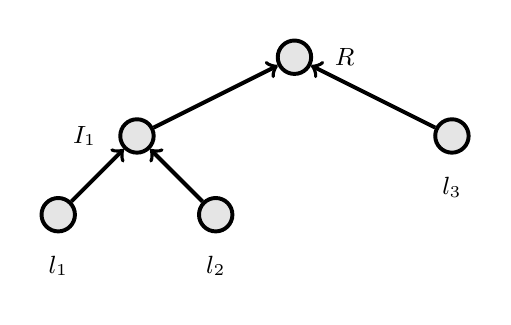
\begin{tikzpicture}
        [level distance=10mm,
        every node/.style={fill=gray!20,draw=black,circle,line width=0.5mm,inner sep=1.5mm},
        edge from parent/.style={<-,draw},
        level 1/.style={sibling distance=40mm,line width=0.5mm,nodes={fill=gray!20}},
        level 2/.style={sibling distance=20mm,nodes={fill=gray!20}},
        level 3/.style={sibling distance=10mm,nodes={fill=gray!20}}]
        \node[label={right:\small $R$}] {}
            child {node[label={left:\small $I_1$}] {}
              child {node[label=south:{\small $l_1$}] {}}
              child {node[label=south:{\small $l_2$}] {}}
            }
            child {node[label={south:\small $l_3$}] {}};
        \end{tikzpicture}
  \end{figure}

  \textit{Submission.}
  You must include the file \texttt{proof.json} in your repository.  
  This file must contain a valid proof for a leaf that you created in the previous task.

  If you were not able to create a leaf yourself, you may use someone else's leaf (but not the proof example).

  The file \texttt{proof\_example.json} contains a valid proof for the actual tree.
  I recommend that you use it to validate your own implementation.

  \textit{Fallback options.}
  If you cannot implement a dynamic proof generation algorithm:
  \begin{itemize}
    \item Compute the intermediate hashes manually and hardcode them in your script.
    Explain it in your report.
    \item If you cannot compute the proof, describe in your report which nodes (and positions) would theoretically be required.
  \end{itemize}
\end{task}

\begin{task}{Extending this assignment}
  TBD SHA256 length extension for authentication.
\end{task}

\end{document}
